%
% For tracking purposes - this is V2.0 - May 2012

\documentclass{sig-alternate-05-2015}

\usepackage[colorinlistoftodos,obeyFinal]{todonotes}                           
%\usepackage{caption}
\usepackage{fainekos-macros}
\usepackage[]{algorithm2e}
\usepackage{amsmath} % assumes amsmath package installed
\usepackage{amssymb}  % assumes amsmath package installed
\usepackage{graphicx}
\usepackage{tikz}
\usetikzlibrary{arrows}
\usepackage{ifthen}
\usepackage{mathtools}
\usepackage{stmaryrd}
\usepackage{csquotes}
\usepackage{xargs}                      % Use more than one optional 
\usepackage{subcaption}
%\usepackage[pdftex,dvipsnames]{xcolor}  % Coloured text etc. 
\usepackage[obeyFinal]{todonotes}

\newcommand{\rob}{\rho}
\newcommand{\robf}{\rho_{\formula}}
\newcommand{\robfa}{\rho_{\formula_1}}
\newcommand{\robfb}{\rho_{\formula_2}}
\newcommand{\srob}{\tilde{\rob}}
\newcommand{\srobf}{\srob_\formula}
\newcommand{\smax}{\widetilde{\max}}
\newcommand{\smin}{\widetilde{\min}}
\newcommand{\sdist}{\mathbf{dist}_\varepsilon}

\newcommand{\sd}{\rho}
\newcommand{\bs}[2]{\ll\!#1,#2\!\gg}
\newcommand{\rd}[2]{\ll\!#1,#2\!\gg_\Re}
\newcommand{\rs}[2]{\ensuremath{\llbracket #1,#2 \rrbracket}}
\newcommand{\cl}[1]{\overline{#1}}
\newcommand{\Ltf}{\Lc_t(\formula)}
\newcommand{\Ltnp}{\Lc_t(\lnot p)}
\newcommand{\Ltp}{\Lc_t(p)}
\newcommand{\Lrf}{\Lc_{\Re_\Fc}}

% Control spacing...
%\setlength{\marginparwidth}{4cm}
%\setlength{\textfloatsep}{2pt}
%\linespread{0.97}
%\thickmuskip=0mu

\begin{document}

\CopyrightYear{2017} \setcopyright{acmcopyright}
\conferenceinfo{ICCPS '17,}{April 18--21, 2017, Pittsburgh, Pennsylvania, USA.}
\isbn{978-1-4503-3955-1/16/04}\acmPrice{\$15.00}
\doi{http://dx.doi.org/10.1145/2883817.2883841}
%Authors, replace the red X's with your assigned DOI string.

\title{Smooth Operator: Control Using the Smooth Robustness of Temporal Logic}

\author{
	% 1st. author
	\alignauthor
	Three little piggies\\
	\affaddr{Department of Electrical and Systems Engineering}\\
	\affaddr{University of Pennsylvania, Philadelphia, PA, USA}\\
	\email{\{piggies1,2,3\}@seas.upenn.edu}%
}


\maketitle
\begin{abstract}
	
\end{abstract}
\section{Introduction}
\label{sec:intro}
The errors in Cyber Physical Systems (CPS) can affect both the cyber components (e.g., software bugs) and physical components (e.g., sensor failures and attacks) of a system.
To deal with unforeseen problems, the system must be controlled at runtime such that it not only satisfies its design specifications, but it satisfies them robustly.
This can give a margin of maneuvarability to the system during which it addresses the unforeseen problem.
Since these problems are, by definition, unforeseen and unmodeled and only detected by their effect on the output, the notion of robustness must be computable using only the output behavior of the system.
%
The \textit{robustness of Metric Temporal Logic specifications} \cite{Fainekos2006_TLVerifSimu,Donze2010} is a rigorous notion that has been used successfully for the verification of automotive systems, medical devices, and general CPS.
In details, MTL is a formal language for expressing complex reactive requirements with time constraints.
Given a specification $\formula$ written in MTL and a system execution $\sstraj$, the robustness $\robf(\sstraj)$ of the spec relative to $\sstraj$ measures two things:
its sign tells whether $\sstraj$ satisfies the spec ($\robf(\sstraj) > 0$) or falsifies it (i.e., violates it, $\robf(\sstraj) <0$).
Its magnitude $|\robf(\sstraj)|$ measures how \textit{robustly} the spec is satisfied or falsified.
Namely, any perturbation to $\sstraj$ of size less than $|\robf(\sstraj)|$ will not cause its truth value to change.
Thus, the control algorithm can \textit{maximize} the robustness over all possible control actions to determine the next control input.
Unfortunately, the robustness function $\robf$ is hard to work with.
In particular, it is non-differentiable, so we have to resort to heuristics or costly non-smooth optimizers. 
This makes its optimization a challenge - indeed, most existing approaches treat it as a black box and apply heuristics to its optimization.

\textbf{In this work, we designed and implemented smooth (infinitely differentiable) approximations to the robustness function of arbitrary MTL formulae, which can be made arbitrarily close to the true robustness.}
This allows us to run powerful and rigorous off-the-shelf gradient descent optimizers.
Here, we use the SQP optimizer, which offers convergence guarantees to the function's (local) minima under certain conditions, and has been optimized so it outperforms heuristics that don't have access to the objective's gradient information.

We demonstrate that the resulting control algorithm performs better than current heuristics, and better than the approach presented in \cite{Raman14_MPCSTL} and subsequent papers on two example systems.
The approach in \cite{Raman14_MPCSTL}, implemented in the tool BluSTL, formulates the robustness maximization problem as a Mixed Integer Linear Programming (MILP) (for linear systems) and uses a MILP solver to solve them.
%The resulting MILP and used a Mixed Integer Linear Program (MILP) has $O(N\cdot|P|)$ binary variables (where $N$ is the number of samples in the trajectory over which we optimize and $|P|$ is the number of predicates, and $O(N\cdot |\formula|)$ continuous variables.
MILPs are NP-hard, and the sophisticated heuristics used to mitigate this make it hard to characterize their runtimes, which is important in control - see examples in \cite{Raman14_MPCSTL}.

This abstract presents the results of the comparison to BluSTL, which represents the state-of-the-art.


\section{Robustness of MTL formulae}
\label{sec:robust semantics}

Consider a discrete-time dynamical system $\Sys$ given by 
\begin{equation}
\label{eq:xt}
x_{t+1} = f(x_t,u_t)
\end{equation}
where $x \in X \subset \Re^n$ is the state of the system and $u \in U \subset \Re^m$ is its control input.
The system's initial state $x_0$ takes value from some initial set $X_0 \subset \Re^n$.
Given an initial state $x_0$ and a control input sequence $\inpSig = (u_0,u_1,\ldots), u_t \in U$, a trajectory of the system is the unique sequence of states $\sstraj = (x_0,x_1,\ldots)$ s.t. for all $t$, $x_t$ is in $X$ and it obeys \eqref{eq:xt} at every time step.
We will use $\TDom$ to abbreviate the time domain $\{0,1,2,\ldots\}$.
All temporal intervals that appear in this paper are discrete-time, e.g. $[a,b]$ means $[a,b] \cap \TDom$. 
For an interval $I$, we write $t+I = \{t+a \such a \in I\}$.
The set of subsets of a set $S$ is denoted $\Pc(S)$.
The signal space $\SigSpace$ is the set of all signals $\sstraj: \TDom \rightarrow X$.
The max operator is written $\sqcup$ and min is written $\sqcap$.

\subsection{Metric Temporal Logic}
\label{sec:mtl}
The controller of $\Sys$ is designed to make the closed loop system \eqref{eq:xt} satisfy a specification expressed in Metric Temporal Logic (MTL)~\cite{Ouaknine08_RecentResultsMTL}.
MTL allows one to formally express complex reactive specifications, beyond stability, trajectory tracking and the like.
%See examples \eqref{eq:rule1mtl} and \eqref{eq:rule3mtl}.

Formally, let $AP$ be a set of atomic propositions, which can be thought of as point-wise constraints on the state of the system.
An MTL formula $\formula$ is built recursively from the atomic propositions using the following grammar:
\[\formula \defeq \top|p|\neg \formula | \formula_1 \lor \formula_2 | \formula_1 \land \formula_2 | \formula_1 \until_I \formula_2\]
where $I \subset \Re$ is a time interval.
Here, $\top$ is the Boolean True, $p$ is an atomic proposition, $\neg$ is Boolean negation, $\lor$ and $\land$ are the Boolean OR and AND operators, respectively, and $\until$ is the Until temporal operator.
Informally, $\formula_1 \until_I \formula_2$ means that $\formula_1$ must hold \textit{until} $\formula_2$ holds, and that the hand-over from $\formula_1$  to $\formula_2$ must happen sometime during the interval $I$.
The implication ($\implies$), Always ($\always$) and Eventually ($\eventually$) operators can be derived using the above operators.

Formally, the \textit{pointwise semantics} of an MTL formula define what it means for a system trajectory $\sstraj$ to satisfy the formula $\formula$.
Let $\Oc: AP \rightarrow \Pc(X)$ be an \textit{observation} map for the atomic propositions.
The boolean truth value of a formula $\formula$ w.r.t. the trajectory $\sstraj$ at time $t$ is defined recursively.
\begin{definition}[MTL semantics]
	\label{def:boolean sat}
	\begin{eqnarray*}
		\label{eq:boolean sat}
		(\sstraj,t) \models \top &\Leftrightarrow& \top
		\\
		\forall p \in AP, (\sstraj, t) \; \models_\Oc p &\Leftrightarrow& x_t \in \Oc(p)
		\\
		(\sstraj,t) \models_\Oc \neg \formula&\Leftrightarrow& \neg (\sstraj,t) \models_\Oc \formula
		\\
		(\sstraj,t) \models_\Oc \formula_1 \lor \formula_2 &\Leftrightarrow& (\sstraj,t) \models_\Oc \formula_1 \lor (\sstraj,t) \models_\Oc \formula_2
		\\
		(\sstraj,t) \models_\Oc  \formula_1 \land \formula_2&\Leftrightarrow& (\sstraj,t) \models_\Oc \formula_1 \land (\sstraj,t) \models_\Oc \formula_2
		\\
		(\sstraj,t) \models_\Oc \formula_1 \until_I \formula_2 &\Leftrightarrow& \exists t' \in t+I .  (\sstraj,t') \models_\Oc \formula_2  
		\\
		&& \, \land \forall t'' \in (t,t'), \;\; (\sstraj,t'') \models_\Oc \formula_1 
	\end{eqnarray*}
\end{definition}
As $\Oc$ is fixed in this paper, we drop it from the notation.
We say $\sstraj$ satisfies $\formula$ if $(\sstraj,0) \models \formula$.
All formulas that appear in this paper have bounded temporal intervals: $ 0\leq \inf I < \sup I < +\infty$.
To evaluate whether such a formula $\formula$ holds on a given trajectory, only a finite-length prefix of that trajectory is needed.
Its length can be upper-bounded by the \textit{horizon} of $\formula$, $hrz(\formula)$, calculable as shown in~\cite{Dokhanchi14_OnlineMonitoring}. 
For example, the horizon of $\eventually_{[2,4]}p$ is 6.

\subsection{Robust semantics of MTL}
\label{sec:rob sem}
Designing a controller that satisfies the MTL formula $\formula$\footnote{Strictly speaking, a controller such that the closed-loop satisfies the formula.} is not always enough.
In a dynamic environment, where the system must react to new unforeseen events, it is useful to have a margin of maneuverability.
That is, it is useful to control the system such that we \textit{maximize} our degree of satisfaction of the formula.
When unforeseen events occur, the system can react to them without violating the formula.
This degree of satisfaction can be formally defined and computed using the robust semantics of MTL.
Given a point $x \in X$ and a set $A \subset X$, $\dist(x,A) \defeq \inf_{a \in \cl{A}}|x-a|_2$ is the distance from $x$  to the closure $\cl{A}$ of $A$.
\begin{definition}[Robustness\cite{FainekosP09tcs}]
	\label{def:robustness estimate}
	The \emph{robustness} of $\varphi$ relative to $\sstraj$ at time $t$ is recursively defined as 
	\begin{eqnarray*}
		\label{eq:robustness estimate}
		\rob_{\top} (\sstraj,t) &=& +\infty
		\\
		\forall p \in AP, \;  \rob_{p} (\sstraj,t) &=& \left \lbrace \begin{matrix}
			\dist(\stPt_t, \stSet \setminus \Oc(p)), &\text{if } \stPt_t \in \Oc(p)
			\\
			-\dist(x_t, \Oc(p)), &\text{if } \stPt_t \notin \Oc(p)						
		\end{matrix} \right.
		\\
		\rob_{\lnot \formula} (\sstraj,t) &=& - \rob_{\formula} (\sstraj,t)
		\\
		\rob_{ \formula_1 \lor \formula_2} (\sstraj,t) &=& \rob_{\formula_1} (\sstraj,t) \sqcup \rob_{\formula_2} (\sstraj,t) 
		\\
		\rob_{ \formula_1 \land \formula_2} (\sstraj,t) &=& \rob_{\formula_1} (\sstraj,t) \sqcap \rob_{\formula_2} (\sstraj,t) 
		\\
		\rob_{ \formula_1 \until_I \formula_2} (\sstraj,t) &=& \sqcup_{t' \in t+_{\TDom}I} \left(\rob_{\formula_2} (\sstraj,t') \bigsqcap \right.
		\\
		&& \left. \sqcap_{t'' \in [t,t')}   \rob_{\formula_1} (\sstraj,t'') \right) 
	\end{eqnarray*}
	When $t=0$, we write $\robf(\sstraj)$ instead of $\robf(\sstraj,0)$.
\end{definition}

\section{Smooth approximation}
\label{sec:smooth apx}
\newcommand{\fe}{f_\varepsilon}

In this section, we come up with an infinitely differentiable approximation for robustness and obtain bounds on the approximation error. We start by stating the problem we want to solve, and why the smooth approximation is helpful.
\subsection{The need for smoothing}
\label{sec:need for smoothing}
Let $\formula$ be an MTL formula with horizon $N$.
We aim to solve the following control problem $P_\rob$.
\begin{subequations}
\label{eq:general_ctrl}
\begin{align}
P_\rob:\, \max\, & \rob_{\formula}(\sstraj) - \gamma \sum_{k=0}^{N-1} l(x_{k+1},u_{k}) \label{eq:general ctrl obj}\\
\text{s.t. } & x_{k+1} = f(x_k,u_k), \, \forall k=0,\dotsc,N-1 \label{eq:general ctrl dyn}\\
 & x_k \in X, \, \forall k=0,\dotsc,N \label{eq:general ctrl X}\\
 & u_k \in U, \, \forall k=0,\dotsc,N-1 \label{eq:general ctrl U}\\
 & \delta \rob_{\formula}(\sstraj) \geq 0 \label{eq:general ctrl pos rob}
\end{align}
\end{subequations}

We want to use established, powerful gradient descent algorithms \cite{Polak97_Optim}, rather than heuristics like Simulated Annealing \cite{kirkpatrickV_SA83}. 
In the above formulation, $l(x_{k+1},u_{k})$ is a system specific control cost, e.g. the LQR cost $x_k'Qx_k + u_k'Ru_k$. $\gamma \geq 0$ is weighting parameter, which is a design choice. $X$ and $U$ define constraints on the state $x$ and control $u$ respectively. $f$ represents the dynamical system, with $x$ as the state and $u$ as inputs. Finally, the last constraint enforces $\rob \geq 0$, i.e. the specification is satisfied. 
$\delta$ here is a binary design choice, $1$ if the constraint is meant to be enforced, $0$ otherwise.
We will need to assume that $f$ is twice Lipschitz continuously differentiable and that its gradient $f_u$ has maximum row rank.

Gradient descent algorithms typically offer convergence guarantees to the function's minima, have known convergence rates for certain function classes, and have been optimized so they outperform heuristics that don't have access to the objective's gradient information.
Moreover, they usually have a fewer number of parameters to be set by the user, and important issues like step-size selection are rigorously addressed.

To apply gradient descent methods, we require a differentiable objective function. 
Our objective function, $\robf$, is non-differentiable, because it uses the distance, max, and min functions, all of which are non-differentiable.
One may note that these functions are all differentiable almost everywhere (a.e.).
That is, the set of points in their domain where they are non-differentiable has measure 0 in $\Re^n$. 
Therefore, by measure additivity, the composite function $\robf$ is itself differentiable almost everywhere.
Thus, one may be tempted to `ignore' the singularities (points of non-differentiability), and apply gradient descent to $\robf$ anyway.
The rationale for doing so is that sets of measure 0 are unlikely to be visited by gradient descent, and thus don't matter. 
However, as we show in the next example, the lines of singularity (along which the objective is non-differentiable) can be  precisely the lines along which the objective increases the fastest.
See also \cite{Cortes08_Discontinuous}.
Thus they are consistently visited by gradient descent, after which it fails to converge because of the lack of a gradient.


\begin{exmp}
	\label{ex:cluster nondiff}
	A simple example illustrates how gradient descent gets stuck at singularities.
	We use Sequential Quadratic Programming (SQP) \cite{Polak97_Optim} to maximize the robustness of $\formula = \neg (x \in U)$, where $U=[-1,1]^2$ is the unsafe red square in Fig.~\ref{fig:DumbExample}.
	In this case, $\robf$ is simply $\dist(x_0,U)$, the distance of the first trajectory point to the set.
	The search space is $[-2.5,2.5]^2$ (big grey square in Fig. \ref{fig:DumbExample}). 
	The most robust point is $x^* = [2.5,2.5]$ (green `+' in figure), being furthest from the unsafe set.
	We initialize the SQP at $x_0=[0,0]$. 
	SQP generates iterates (blue circles) \textit{on the line of singularity} connecting $[1,1]$ to $x^*$ and ultimately gets stuck at $x=[1,1]$.
	That's because along the line, the gradient does not exist and attempts by SQP to approximate it numerically fail, prompting it to generate smaller and smaller step-sizes for the approximation.
	Ultimately, SQP aborts due to the step-size being too small, and concludes it is at a local minimum.
	
\begin{figure}[t]
\centering
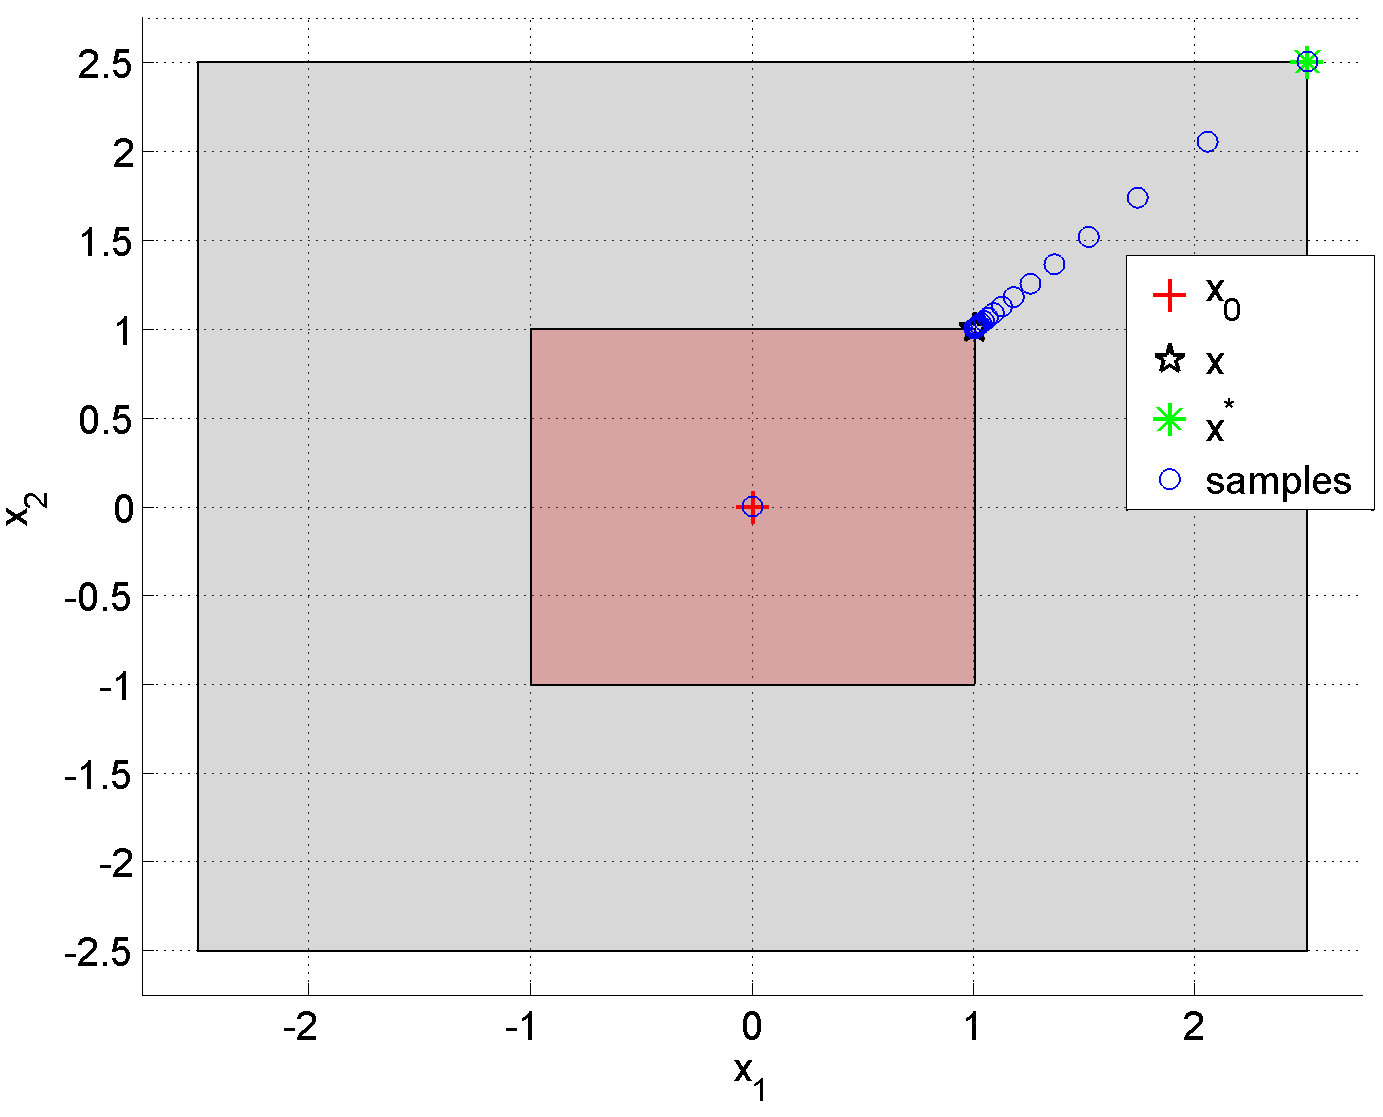
\includegraphics[width=0.49\textwidth]{figures/DumbOptEx_scissored}
\vspace{-20pt}
\caption{{\small Iterates of SQP for Example \ref{ex:cluster nondiff}. Colors in online version.}}
\vspace{-10pt}
\label{fig:DumbExample}
\end{figure}

\end{exmp}

\subsection{Approximating the distance function}
\label{sec:dist smoothing}
To create a smooth approximation to $\robf$, we use smooth approximations to each of its non-differentiable components: the set-distance, min, and max functions.

\begin{figure}[t!]
	\centering
	\begin{subfigure}[t]{0.25\textwidth}
		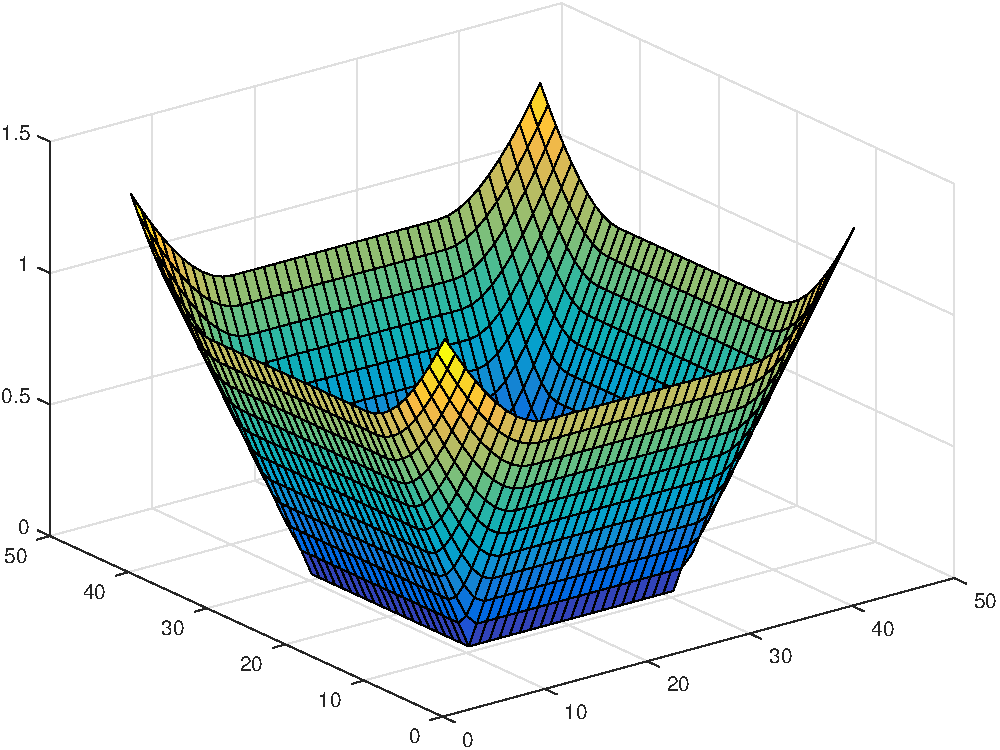
\includegraphics[height=1.2in]{figures/smoothDist2d}
		\caption{Smoothed function}
	\end{subfigure}%
	~
	\begin{subfigure}[t]{0.25\textwidth}
		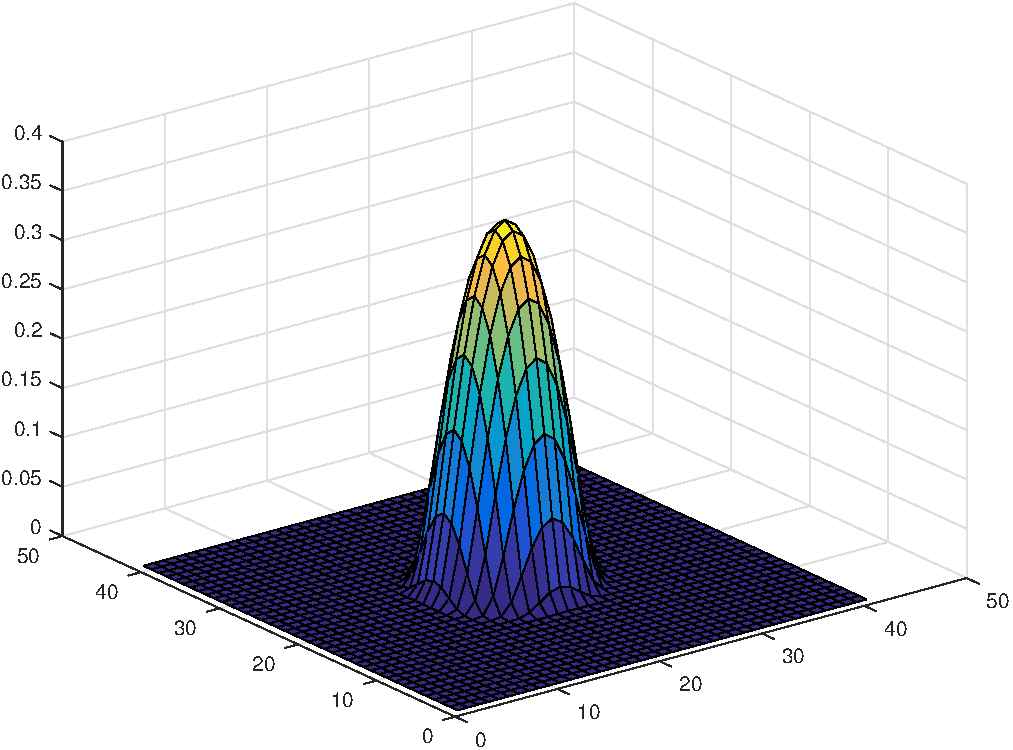
\includegraphics[height=1.2in]{figures/kernelG}
		\caption{Function $g$}
	\end{subfigure}
	\caption{{\small Smoothed 2-d distance function to a square in the x-y plane, and the function $g$ used to smoothen it.}}
	\vspace{-20pt}
	\label{fig:smooth2d}
\end{figure}

Recall that for a set $U \subset \Re^n$, $\dist(x,U) = \inf_{a \in \cl{U}} |x-a|_2$, where $|\cdot|_2$ is the Euclidian norm.
This function is globally Lipschitz with Lipschitz constant 1 and therefore differentiable almost everywhere (Rademacher's theorem), and has a second derivative almost everywhere if $U$ is convex (Alexandrov's theorem) \cite{MakelaN92book}.

It is well-known that if we convolve an a.e.-differentiable function with a smooth kernel, the output function no longer has those singularities.
We give an example of such a construction, which lays the groundwork for explaining the more general wavelet-based smoothing we use in the experiments.
$C^\infty(\Re^n)$ is the class of functions that are infinitely differentiable in $\Re^n$.
\begin{theorem}
	\label{thm:ge smoothing}
	Consider the globally Lipschitz function $f:\Re^n \rightarrow \Re$ with Lipschitz constant $L_f$.
	Let $g: \Re^n \rightarrow \Re_+$ be a non-negative $C^\infty(\Re^n)$ function that integrates to 1 and is supported on the unit ball:
	$\int_{\Re^n}g(x)dx = 1$, $g(x) = 0$ if $x \notin B(0,1)$.
	Define $g_\varepsilon = \varepsilon^{-n}g(x/\varepsilon)$ and
	\[f_\varepsilon(x) = f *g_\varepsilon(x) = \int_{\Re^n}f(y)g_\varepsilon(x-y)dy\]
	Then $\fe$ is infinitely differentiable, its Lipschitz constant $L_{\fe} \leq L_f$ and $\|f-\fe\|_\infty \leq L_f \varepsilon$.
\end{theorem}
\begin{proof}
	Clearly, $\fe$ is $C^\infty$: $g_\varepsilon \in C^\infty$ and the integrand in the above convolution is differentiable w.r.t. $x$, so it holds that $\fe'(x) = \int{f(y)\partial g_\varepsilon(x-y)/\partial x dy}$.
	
	Convolution is commutative so $f_\varepsilon(x) = \int_{\Re^n}f(x-y)g_\varepsilon(y)dy$.
	Let $x' \in \Re^n$, then 
	\begin{eqnarray*}
	|\fe(x)-\fe(x')| &=& |\int_{\Re^n} f(x-y)g_\varepsilon(y) - f(x'-y)g_\varepsilon(y) dy|
	\\
	&\leq & \int_{\Re^n} g_\varepsilon(y)|f(x-y) - f(x'-y)| dy
	\\
	& = & L_f|x-x'| \int_{\Re^n} \varepsilon^{-n} g(y/\varepsilon) dy
	\\
	&= &L_f|x-x'| \int_{\Re^n} \varepsilon^{-n} g(y') \varepsilon^ndy'
	\\
	&=& L_f|x-x'| \implies L_f \leq L_{\fe}
	\end{eqnarray*}
	
	Finally, 
	\begin{eqnarray*}
	|\fe(x)-f(x)| &=& \left|\int_{\Re^n}f(x-y)g_\varepsilon(y)dy - \int_{\Re^n}f(x)g(y)dy\right|
	\\
	&=& \left|\int_{\Re^n}f(x-\varepsilon y)g(y)dy - \int_{\Re^n}f(x)g(y)dy\right|
	\\
	&\leq& \int_{B(0,1)}|f(x- \varepsilon y) - f(x)|g(y)dy	
	\\
	&\leq & \int_{B(0,1)}L_f | \varepsilon y| g(y)dy \leq L_f \varepsilon
	\end{eqnarray*}
	In particular, $\|f-\fe\|_\infty \rightarrow 0$ as $\varepsilon \rightarrow 0$.
\end{proof}
Fig.~\ref{fig:smooth2d} shows the distance function $\dist(\cdot,U)$ where $U$ is a square in the plane, smoothed by convolving with kernel $g_{\varepsilon}$ obtained from the shown function. 
We used $\varepsilon = 0.001$, and the actual approximation error $\|f-\fe\|_\infty$ is less than 1e-15.
Parameter $\varepsilon$ controls how peaked or flat $g_\varepsilon$ is: a large $\varepsilon$ gives a peaked kernel which yields better local approximation, but the max error decreases towards 0 slower.

%\todo[inline]{because lip cnt is bounded by that of f, this says that it's a conservative apx? if d is -ve and decreasing, $d_\varepsilon$ decreases less and if d is +ve and increasing, $d_e$ increases less.}

\subsection{Wavelet approximations}
\label{sec:waveletApx}

Wavelets can be viewed as a generalization of the kernel $g_\varepsilon$ of the previous section to a whole family of kernels, obtained by translations and dilations of one function called the `mother wavelet' $\psi$: $\psi_{k,j}(x) = \sqrt{2^{-j}}\psi(2^{-j}(x-k))$  \cite{MallatBook}.
They are used extensively in signal processing, as they have very good approximation properties, including fast convergence and multi-scale analysis.
See \cite{MallatBook}.
In the experiments in the rest of this paper, we used the Meyer wavelets. 
Specifically
\todo[inline]{Yash, meyer}
 

\subsection{Smooth max and min}
\label{max min smoothing}
We use the following standard smooth approximations of $m$-ary max and min.
Let $k \geq 1$.
\begin{eqnarray}
	\label{eq:soft max min}
	\smax_k(a_1,\ldots,a_m) &\defeq& \frac{1}{k} \ln(e^{ka_1}+\ldots+e^{ka_m})
	\\
	\smin_k(a_1,\ldots,a_m) &\defeq& -\smax(-a_1,\ldots,-a_m)
\end{eqnarray}
Suppose $k=1$ and that $a_1$ is the largest number.
Then $e^{a_1}$ is even larger than the other $e^{a_i}$'s, and dominates the sum. 
Thus $\smax_1(\mathbf{a}) \approxeq \ln e^{a_1} = a_1 = \max(\mathbf{a})$.
If $a_1$ is not significantly larger than the rest, the sum is not well-approximated by $e^{a_1}$ alone.
To counter this, the scaling factor $k$ is used: it amplifies the differences between the numbers.
It holds that for any set of $m$ reals,
\begin{eqnarray}
\label{eq:smooth max error}
0 \leq \smax_k(a_1,\ldots,a_m) -\max(a_1,\ldots,a_m) \leq \ln(m)/k
\\
0 \leq \min(a_1,\ldots,a_m) -\smin_k(a_1,\ldots,a_m) \leq \ln(m)/k
\end{eqnarray}
Indeed, the error of smooth max can be bounded as follows.
Assume $a_1$ is the largest number, then 
\begin{eqnarray*}
\varepsilon_M &\defeq& \smax_k(\mathbf{a}) - a_1 =  \frac{\ln(\sum_ie^{ka_i})-ka_1}{k}
\\
&=& k^{-1}\ln\left(\frac{\sum_ie^{ka_i}}{e^{ka_1}}\right) \leq k^{-1}\ln \left(\frac{me^{ka_1}}{e^{ka_1}}\right)
\\
&=&\frac{\ln m}{k}
\end{eqnarray*}
It is also clear from what preceded that $\varepsilon_M \geq 0$.
The maximum error is achieved when all the $a_i$'s are equal.
\subsection{Overall approximation}
\label{sec:overall apx}
Putting the pieces together, we obtain the approximation error for the robustness of any MTL formula.
\begin{theorem}
	\label{thm:total apx error}
	Consider an MTL formula $\formula$ and reals $\varepsilon > 0$ and $k \geq 1$. 
	Define the \textit{smooth robustness} $\srobf$, obtained by substituting $\sdist_{\varepsilon}$ for $\mathbf{dist}$, $\smax_k$ for $\max$, and $\smin_k$ for $\min$, in Def. \ref{def:robustness estimate}.
	Then for any length-$N$ trajectory $\sstraj$, it holds that
	\[|\robf-\srobf| \leq \delta_\formula\]
	where $\delta_\formula$ is
	(a)independent of the evaluation time $t$, and 
	(b) goes to 0 as $\varepsilon \rightarrow 0$ and $k \rightarrow \infty$.
%	\[|\robf-\srobf| \leq |\formula| \cdot \max(\varepsilon,\ln(m)/k)\]
%	where $m$ is the length of the longest temporal interval appearing in $\formula$ and $|\formula|$ is the size of the formula, i.e. the number of operators that appear in it.
\end{theorem}
\begin{proof}
	We will prove a stronger result that implies the theorem.	
%	Define $\delta_\formula \in \Re_+$ inductively: 
%	$\delta_\top = 0, \delta_p = \varepsilon$, $\delta_{\neg \formula} = \delta_\formula$, 
%	$\delta_{\formula_1 \lor \formula_2} = \delta_{\formula_1 \land \formula_2} = \delta_{\formula_1} \sqcup \delta_{\formula_2} + \ln(2)/k$,
%	$\delta_{\formula_1 \until_{[a,b]} \formula_2}  = \delta_{\formula_1} \sqcup \delta_{\formula_2} + \ln(b-a)/k$.
%	Noting that $\delta_\formula \leq |\formula| \cdot \max(\varepsilon,\ln(m)/k)$, it suffices to show that the error is upper-bounded by $\delta_\formula$.
	When $\sstraj$ or $t$ are clear from the context, we will drop them from the notation.
	
	The proof is by structural induction on $\formula$, and works by carefully characterizing the approximation error.
	The case $\formula = \top$ is trivial.
	
\underline{Case $\formula = p \in AP$.}
$\robf(\sstraj,t)$ is given by either $\dist{x_t}{\Oc(p)}$ or $-\dist{x_t}{\Oc(p)}$, and 
$\srobf(\sstraj,t)$ is given by either $\sdist_\varepsilon(x_t,\Oc(p))$ or $-\sdist_\varepsilon(x_t,\Oc(p))$, respectively.
Either way, $|\srobf(\sstraj,t) - \robf(\sstraj,t)| \leq \varepsilon$.
Indeed, $\varepsilon$ satisfies the conditions on $\delta_\formula$.

\underline{Case $\formula = \neg \formula_1$} 
$|\rob_{\neg \formula_1}(\sstraj,t)-\srob_{\neg \formula_1}(\sstraj,t)| = |-\rob_{\formula_1}(\sstraj,t) + \rob_{ \formula_1}(\sstraj,t)|  \leq \delta_{\formula_1}$, and $\delta_{\formula_1}$ satisfies (a)-(b) by induction hypothesis.

\underline{Case $\formula = \formula_1 \lor \formula_2$}.
If the same sub-formula $\formula_i$ achieves the max for both $\rob_{\formula_1}(\sstraj,t) \sqcup \rob_{\formula_2}(\sstraj,t)$ and $\srob_{\formula_1}(\sstraj,t) \sqcup \srob_{\formula_2}(\sstraj,t)$, then by induction hypothesis we immediately obtain 
$|\robf(\sstraj,t)-\srob(\sstraj,t)|  \leq \delta_{\formula_i} \leq \delta_{\formula}$.

Otherwise if, say, $\robf = \rob_{\formula_1}$ and $\srobf = \srob_{\formula_2}$ then
\[\robfa -\delta_{\formula_1} \leq \srob_{\formula_1} \leq \srob_{\formula_2} \implies \robfa-\srob_{\formula_2} \leq \delta_{\formula_1}\]
Also 
\[\srob_{\formula_2} \leq \robfb+\delta_{\formula_2} \leq \robfa + \delta_{\formula_2} \implies -\delta_{\formula_2} \leq \robfa - \srob_{\formula_2}\]
Therefore
\begin{equation*}
\label{eq:inter}
-(\delta_{\formula_1} \sqcup \delta_{\formula_2})\leq \robfa - \srob_{\formula_2}\leq \delta_{\formula_1} \sqcup \delta_{\formula_2} \Leftrightarrow |\robfa - \srob_{\formula_2}|\leq \delta_{\formula_1} \sqcup \delta_{\formula_2}
\end{equation*}
Similarly, if $\robf = \rob_{\formula_2}$ and $\srobf = \srob_{\formula_1}$, we have $|\robfb - \srob_{\formula_1}|\leq  \delta_{\formula_1} \sqcup \delta_{\formula_2}$.
So in all cases, 
\[|\robfa \sqcup \robfb - \srob_{\formula_1} \sqcup \srob_{\formula_2}|\leq \delta_{\formula_1} \sqcup \delta_{\formula_2}\]
Therefore by the triangle inequality and \eqref{eq:smooth max error}
\[|\robfa \sqcup \robfb - \smax_k(\srob_{\formula_1} , \srob_{\formula_2})|\leq  \delta_{\formula_1} \sqcup \delta_{\formula_2} + \ln(2)/k  = \delta_\formula\]
Clearly, $\delta_\formula$ satisfied (a)-(b).

The case $\formula_1 \land \formula_2$ is treated similarly.

\underline{$\formula = \formula_1 \until_I \formula_2$.} 
Before proving this case, we will need the following lemma, which is provable by induction on $n$:
\begin{lemma}
	\label{lemma:n-ary apx}
	If $\formula = \formula_1\land \ldots\land \formula_n$ or $\formula = \formula_1\lor \ldots\lor \formula_n$, $n\geq 2$, then 
	$|\robf - \srobf| \leq \sqcup_{1\leq i \leq n}\delta_{\formula_i} + \ln(n)/k$.
\end{lemma}

We now proceed with the proof of the last case.
Recall that $\rob_{ \formula_1 \until_I \formula_2} (\sstraj,t) = \sqcup_{t' \in t+_{\TDom}I} \left(\rob_{\formula_2} (\sstraj,t') \bigsqcap \right.
\\
\left. \sqcap_{t'' \in [t,t')}   \rob_{\formula_1} (\sstraj,t'') \right)$.
Starting with the innermost sub-expression $\rob_\psi \defeq \sqcap_{t'' \in [t,t')}   \rob_{\formula_1} (\sstraj,t'')$, we have, by Lemma \ref{lemma:n-ary apx}
\begin{equation}
\label{eq:robpsi}
|\rob_{\psi}-\srob_\psi| \leq \sqcup_{t'' \in [t,t')}\delta_{\formula_1}^{t''} + \ln(t'-t)/k
\end{equation} 
where $\delta_{\formula_1}^{t''} $ is the bound for approximating $\rob_{\formula_1}(\sstraj,t'')$.
But $\delta_\formula$ does not depend on the time at which the formula is evaluated. 
Therefore the bound in \eqref{eq:robpsi} becomes
\begin{equation}
\label{eq:t'-t}
|\rob_{\psi}-\srob_\psi| \leq \delta_{\formula_1} + \ln(t'-t)/k
\end{equation} 
%
To avoid introducing a dependence on time, we further upper-bound by 
\begin{equation*}
|\rob_{\psi}-\srob_\psi| \leq \delta_{\formula_1} + \ln(hrz(\formula))/k \defeq \delta_\psi
\end{equation*} 
where, recall, $hrz(\formula)$ is the horizon of $\formula$ (see Section \ref{sec:mtl}).

Continuing with the sub-expression $\rob_\alpha = \rob_{\formula_2} (\sstraj,t') \bigsqcap \rob_\psi$, by the induction hypothesis it holds that 
$|\rob_\alpha - \srob_\alpha| \leq \delta_{\formula_2} \sqcup \delta_\psi + \ln(2)/k \defeq \delta_\alpha$.
%
Finally, the top-most max operator introduces the total error 
\begin{eqnarray}
\label{eq:deltaphi until}
|\robf-\srobf| &\leq& \delta_\alpha + \ln(|I|)/k 
\nonumber
\\
&=& \delta_{\formula_2} \sqcup \delta_\psi + \ln(2)/k + \ln(|I|)/k 
\nonumber 
\\
&=& \delta_{\formula_2} \sqcup ( \delta_{\formula_1} + \ln(hrz(\formula))/k )+ \ln(2|I|)/k 
\nonumber
\\
&=&\delta_\formula
\end{eqnarray}
The first inequality obtains from the fact that $\delta_\alpha$ is independent of evaluation time and Lemma \ref{lemma:n-ary apx}.
The bound $\delta_\formula$ obey s (a)-(b).
This concludes the proof.
%if $\formula_1$ is a sub-formula of $\formula$, then $\delta_{\formula_1} \leq \delta_\formula$.
	\end{proof}
	
\begin{rem}
	The proof suggests in \eqref{eq:deltaphi until} that every Until operator increases the error by $+\ln(hrz(\formula))/k$, which may be a large quantity for long-horizon formulas.
	However, a more careful analysis of the accumulation of interval widths $t'-t$, which we upper bounded above by $hrz(\formula)$, reveals that that is not the case.
	Indeed, consider the formula
	\[\formula = \underbrace{(\formula_1 \until_{[a,b]} \formula_2) }_{\psi}\until_{[c,d]} \formula_3\]
	where $\formula_i$ does not contain temporal operators and let $t_\psi$ be the satisfaction time of $\psi$. 
	I.e. it is the time in $[a,b]$ when $\formula_2$ becomes true and `takes over' from $\formula_1$.
	Then, using \eqref{eq:t'-t}, $\delta_{\formula}$ is equal to
	\begin{eqnarray*}
	 && \delta_{\formula_3} \sqcup ( \delta_{\psi} + \ln(t_{\formula_3} - t_\psi)/k )+ \ln(2[d-c])/k 
	\\
	&\leq& \delta_{\formula_3} \sqcup ( \delta_{\psi} + \ln(t_\psi + d - t_\psi)/k )+ \ln(2[d-c])/k 
	\\
	&\leq& \delta_{\formula_3} \sqcup ( \delta_{\psi} + \ln(d)/k )+ \ln(2[d-c])/k 
	\\
	&=& \delta_{\formula_3} \sqcup \left( \underbrace{\delta_{\formula_2} \sqcup ( \delta_{\formula_1} + \ln(b)/k )+ \ln(2[b-a])/k }_{\delta_\psi} + \ln(d)/k \right)
	\\
	&& \quad + \ln(2[d-c])/k 
	\end{eqnarray*}
	The sum of interval widths, such as $\ln(2[b-a])+\ln(2[d-c])$ in this example, gives a \textit{total} $\sum_j\ln(2|I_j|) = \#\until\ln(2) +  \sum\ln(|I_j|)$, where $\#\until$ is the number of times $\until$ appears in $\formula$ and th e$I_j$ are all the temporal intervals. 
	This quantity, in most cases, will actually be smaller than the horizon.
	The sum of interval right endpoints, such as $\ln(b)/k + \ln(d)/k$ in this example, yields $\sum_j \ln(\sup I_j)/k$ \textit{in total}, which is smaller than the horizon.
\end{rem}

%???Indeed, we may view boolean semantics, robust semantics, and smooth robust semantics as lying on one spectrum: 
%in boolean semantics, we use discontinuous (hard) indicator functions for the atomic sets $A = \Oc(p)$: $d^\Be_A(x) = 0$ if $x \in A$, and equals 1 otherwise.
%In robust semantics, this is replaced by a continuous indicator function: $d_A^C(x)$ equals the distance between point $x$ and the set $A$, and thus decreases continuously from positive values (outside the set) to 0 (inside it).
%In the smooth robust semantics we introduce here, we use a smooth indicator function: $d_A^S(x)$ is a differentiable approximation to $d_A^C$, and thus decreases smoothly from positive values to 0.
\section{Case studies}
\label{sec:case study}

We solve a robustness maximization problem for the control of two systems using the following methods.

\begin{itemize}
	\vspace{-5pt}
	\item SOP in (B)oolean and (R)obust modes.
	\vspace{-5pt}
	\item BluSTL in modes (B) and (R).
	\item R-SQP, which uses SQP to optimize the \textit{exact} non-smoothed robustness $\robf$.
	\vspace{-5pt}
	\item SA, which uses Simulated Annealing to optimize $\robf$.%the true robustness
	\vspace{-5pt}
\end{itemize}

%A) Temperature control of a 4-state, single-zone model of a room, with an occupancy dependent comfort specification (similar to \cite{Raman14_MPCSTL}) and B) An Autonomous Centralized Air Traffic Control system for control of two quad-rotors in a constrained airspace with an obstacle, the specification in which corresponds to safely landing the two quad-rotors while following the rules of the airspace. We compare out approach, which consists of gradient descent on the smooth robustness of the specification (via SQP) to A) Simulated Annealing (\cite{}) for robustness maximization and B) Gradient descent on the robustness function (via SQP). 
%\todo[inline]{rather than this intro, just start giving each case study subsection. so lose above paragraph, maybe just one sentence that says "we evaluated the control performance using smooth robustness on a alnging bla and a building bla." Also don't use A and B twice, every time for different things. }

%All methods are implemented in MATLAB, and 
%solving the control problem is preceded by an offline phase which consists of finding the wavelet parameters for the signed distance function approximation for all atomic propositions involving polyhedrons. 
%\todo[inline]{sentence is long and awkward and mixes 2 very different pieces of information. can simply say "we compute the wavelet approimation of the distance function to the sets $\Oc(p)$ off-line"}

For both case studies, we compute the wavelet approximation of the distance function to the sets $\Oc(p)$ off-line. 
Next, we solve the control problem \eqref{eq:general_ctrl} as a single shot, finite horizon constrained optimization. 

The code to reproduce these results can be found at \protect\url{https://github.com/yashpant/SmoothOperator0}. Future release of the code will focus on re-usability of the code and making it handle any system.
%In general, for a real online implementation, the problem can be solved in a receding horizon manner or in a manner where the state and actions of the past are stored an added as constraints at each time step while the look-ahead horizon of the optimization shrinks (similar to \cite{Raman14_MPCSTL}). The problem of which method is suitable for what kinds of specifications is left for future work.
%\todo[inline]{too soon, the control problem hasn't been formulated yet. first forumlate it (or, better, refer to section 4.2), \textit{solve it}, then critique it. Discussion of related work like Vasu's should be after you present what you did, not before}
%\todo[inline]{introduce two numerical examples. Finite horizon control in a single shot, can be applied in a receding/shrinking horizon approach wherever applicable.}


\subsection{HVAC Control of a building for comfort}
%\todo[inline]{skipping for now. i suspect many of my comments for ATC are applicable here, so please apply them as needed}
%caseBldg

We evaluate the control performance of our approach (SR-SQP) and compare it to R-SQP and SA. % of our method on a system with more meaningful dynamics than the point-mass system, 
This is done by testing it on the Heating, Ventilation and Air Conditioning (HVAC) control of a 4-state model of a single zone in a building. Such a model is commonly used in literature for evaluation of predictive control algorithms \cite{Jain2016}. The control problem we solve is similar to the example used in \cite{Raman14_MPCSTL}, where the objective is to bring the zone temperature to a comfortable range when the zone is occupied (given predictions on the building occupancy). The specification is:
\begin{equation}
\label{eq:BldgSpec}
\formula = \always_I(\text{ZoneTemp} \in [22,28])
\end{equation}

Here, $I$ is the time interval where the zone is occupied and the range of temperatures (in Celsius) deemed comfortable is ($[22,28]$). For the control horizon, we consider a 24 hour period, in which the building is occupied from time steps $10$ to $19$ (i.e. $I=[10,19]$), i.e. a 10-hour workday. 

\textit{Note:} In this particular problem, the maximum robustness achievable is $3$, which can be achieved by setting the room temperature at $25$C for the interval $I$. 
With this insight, the problem of maximizing robustness can be solved with a quadratic program with linear constraints and the cost $\sum_{k \in I}({x_4}_k-25)^2$ to be minimized. This indeed results in a trajectory with the global optimal robustness of $3$, but is a method tailored to the particular problem. 

SR-SQP, which is a general purpose technique, results in a robustness which is just $0.02\%$ less than the global optimal value. In the example that follows this one, we take a specification which cannot be trivially turned into a quadratic-program.

\textbf{System dynamics.} The single-zone model, discretized at a sampling rate of 1 hour (which is common in building temperature control) is of the form:
\begin{equation}
\label{eq:bldg_dyn}
x_{k+1} = Ax_{k}+Bu_k+B_dd_k
\end{equation}
Here, $A$, $B$ and $B_d$ matrices are from the hamlab ISE model \cite{VanSchijndel2005}. $x \in \mathbb{R}^4$ is the state of the model, the $4^{th}$ element of which is the zone temperature, the others are auxiliary temperatures corresponding to other physical properties of the zone (walls and facade). The input to the system, $u \in \mathbb{R}^1$, is the heating/cooling energy. $b_d \in \mathbb{R}^3$ are disturbances (due to occupancy, outside temperature, solar radiation). We assume these are known a priori.
%perfect predictions of. Data for the disturbances is obtained for $1^{st}$ April 2000, which is our 24 hours of interest, from \cite{VanSchijndel2005}. 
The control problem we solve is of the form in \eqref{eq:general_ctrl}, with $\gamma$ and $\delta$ both set to zero (correspondingly, not cost for control in BluSTL), and $X=[0,50]^4$, $U=[-1000,2000]$.
%i.e. robustness (smooth, when applicable) is only in the objective, to be maximized. This allows for a fair comparison between the three methods. 
%With respect to the general control problem of \eqref{eq:general_ctrl}, the limits on the states are $X=[0,50]^4$ and on the inputs $U=[-1000,2000]$.

\begin{table}[tb]
\small
\begin{center}
\caption{{\small Runtimes (mean and standard, in seconds) for Smooth Operator (SR-SQP), BluSTL (BlS) and Simulated annealing (SA) over 100 runs with random initial states. Here, (B) means \textit{boolean} mode and (R) means \textit{robust} mode of operation.}}
\vspace{-5pt}
\label{tbl:time_performance_bldg}
\begin{tabular} {|c|c|c|c|}
	\hline
	BlS (B) & SR-SQP (B) & SR-SQP (R) & SA (R) \\ \hline
	 $0.041 \pm 0.002$ &  $\mathbf{0.014 \pm 0.002}$  &  $2.532 \pm 0.26$ & $8.56 \pm 0.31$ \\ \hline 
\end{tabular}	
\end{center}
\end{table}



\textbf{Results.} For comparison across all methods, we run 100 instances of the problem, starting from random initial states $x_0 \in [20,21]^4$. SA, R-SQP and SR-SQP are initialized with the same initial trajectories. The final trajectories after optimization from all methods are shown in Fig.\ref{fig:ZoneTemp} for a particular instance with $x_0 = [21,21,21,21]'$. To reduce clutter, we do not visualize trajectories from SA and R-SQP in \textit{boolean} mode. 

\textbf{Analysis.} In \textit{boolean} mode, SR-SQP, BluSTL, and SA (terminated at $\rob>0$) all find satisfying trajectories across all 100 instances, while R-SQP does not find one for any run and always exits at a local minima. Execution times for SR-SQP and BluSTL are shown in table \ref{tbl:time_performance_bldg}. For SA in \textit{boolean} mode, the run-times have a mean and standard deviation of $3.7s$ and $2.3s$ respectively. R-SQP has run-times in the order of minutes. This is because of the lack of existence of an explicit gradient of $\rob$ and MATLAB's numerical approximation of the gradient slows down the optimization.


In \textit{robust} mode, our method (SR-SQP) and SA both result in trajectories that satisfy $\formula$, with an average robustness of $2.9994$ and $2.8862$ respectively. On the other hand, R-SQP results in a trajectory that does not satisfy $\formula$ ($\rob_{\formula} = -0.1492$), and terminates on a local maxima. Perhaps surprisingly, BluSTL also does not manage to find a satisfying trajectory (average $\rho=-2.71$ for any of the 100 runs. One particular instance is shown in fig. \ref{fig:ZoneTemp}. This could be because the MILP encoding of robustness for this example results in the solver finding local minima which have negative robustness. In terms of run-times, shown in table \ref{tbl:time_performance_bldg}, SR-SQP takes $2.5s$ on average, which is slower than BluSTL, but always finds a trajectory which achieves near global optima of robustness. SA in \textit{robust} mode takes $8.56s$ on average, with a standard deviation of $0.31s$. R-SQP again takes minutes to return a non-satisfying trajectory across all 100 runs. 
%This is possibly due to the lack of existence of a gradient along certain directions, as seen in example \ref{ex:cluster nondiff}.

%\ypcomment{Move to after spec.}

%, while SA gets to a value $3.8\%$ less than the global optima. 
%We use this example to illustrate the applicability of our method, as well as its performance, while adding a word of caution against the use of gradient descent for maximizing the true robustness.
%, even while the gradient of robustness exists \textit{almost everywhere}. 
%In the following example, we take a specification which cannot be trivially turned into a quadratic-program. %without adding tighter constraints than the specification asks for (or binary variables).

\subsubsection{Online implementation} 
%\textbf{Online implementation.} 
Our scheme can also be implemented online in a receding (shrinking) horizon method similar to \cite{Raman14_MPCSTL}. Note that the control horizon in Eq. \ref{eq:general_ctrl} is as at least long as the formula horizon $N$, and evaluating $\srob$ in general requires a trajectory of length $N$. 
For each time step $k=0,\dotsc,N$, we solve the problem of Eq.\ref{eq:general_ctrl} while constraining the variables (the previously applied inputs and states, when applicable) for times steps $<k$ to their actual values. In this scheme, the length of the optimization remains $N$, but the number of free variables keeps on shrinking as $k$ increases. For initializing SR-SQP at each time step, the sequence of inputs (or states) computed at time $k-1$ is used as an initial solution for the optimization at time $k$. 
We implemented this scheme for the HVAC control problem with additional unknown disturbances in the dynamics of the form:
  
\begin{equation}
\label{eq:bldg_dyn_noisy}
x_{k+1} = Ax_{k}+Bu_k+B_dd_k+B_dw_k
\end{equation}

Here, $w_k$ is a uniform random variable centred around the known $d_k$ with a width of $10\%$ of element wise magnitude of $d_k$. This can be thought of as prediction errors in the disturbances like solar radiation and outside temperature. Over 100 runs with random initial states as before, the online application of SR-SQP (in \textit{robust} mode) resulted in an average robustness value of $2.91$. In terms of execution time, the first iteration takes times of the order of those in table \ref{tbl:time_performance_bldg}, and subsequent iterations take a fraction of that time (average for one instance $0.0151s$). This is because we re-use the input sequence at time $k-1$ as an initial guess for the solver at time $k$. Since at the initial time step we have achieved near global robustness maxima, the subsequent SQP optimizations terminate much faster while the formulation takes into account change in the state due to disturbance values by making small changes to the input sequence being computed at time $k>0$. The high value of average robustness and the small execution time per iteration show the applicability of SR-SQP as an online closed loop control method. 

\begin{figure}[t]
\centering
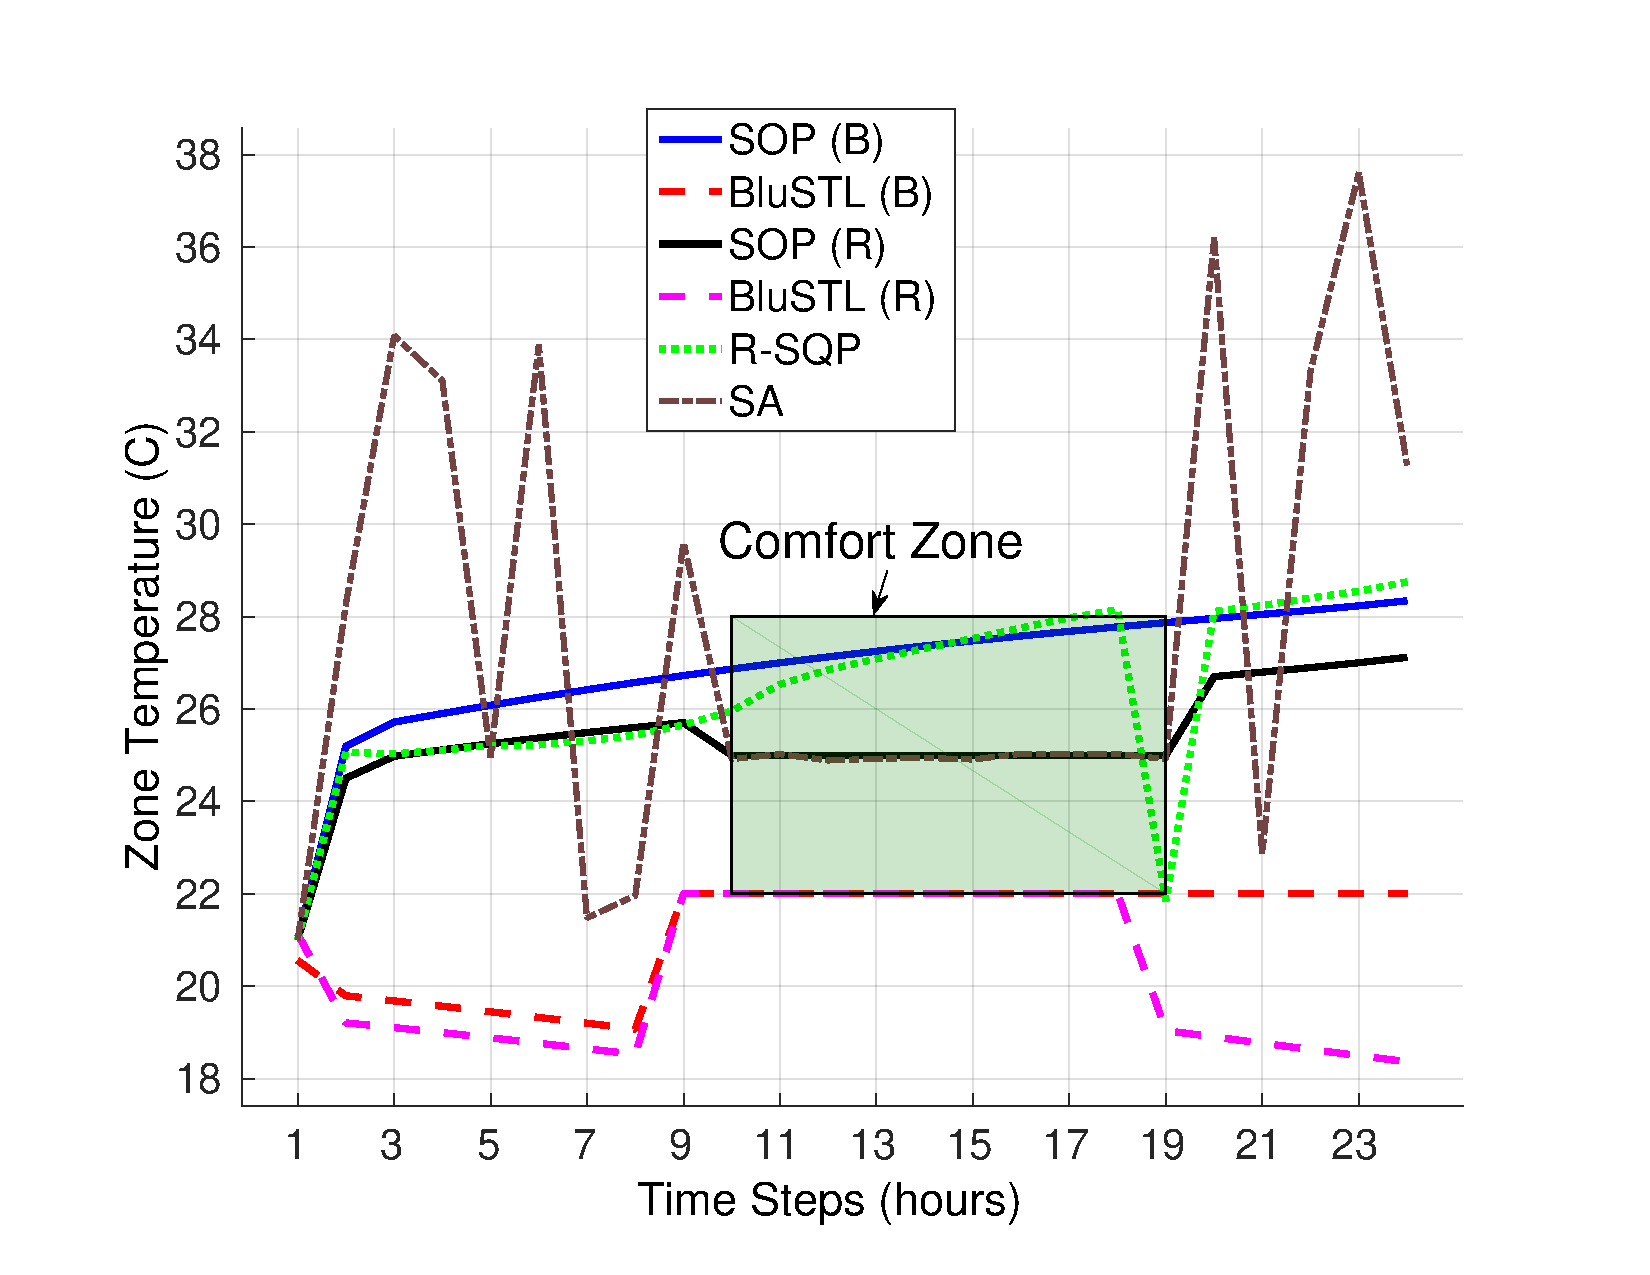
\includegraphics[width=0.49\textwidth]{figures/ZoneTempFinal}
\vspace{-20pt}
\caption{\small{Zone temperatures. The green rectangle shows the comfortable temperature limit of 22-28 C, applicable during time steps 10-19 (when the building is occupied).}}
\label{fig:ZoneTemp}
\vspace{-10pt}
\end{figure}

%1. Single zone building model from ...

%2. Specification for comfort when occupied.

%3. 24 hour look ahead, given disturbances and occupancy. Initial guess (with negative robustness) via solving an LP.

%4. Can be applied in a receding horizon manner. For the given setting, could very well be solved using a linear program asking for temperature between 22-28C for time steps 10 to 19, but we use our method to illustrate how robustness based control can be used to satisfy a specification. The next example (Autonomous ATC) shows control with a specification cannot be trivially translated to a linear program with Polyhedral constraints.

%5. Figure shows room temperature for the 3 methods (other states and disturbances/control in a single figure if necessary)

%6. Table shows robustness of obtained trajectory via the 3 methods. Note, Optimal solution would be temperature of 25C  (robustness of 3) for the occupancy period (if dynamics/constraints would allow it).


%\vspace{-10pt}
\subsection{Autonomous ATC for quad-rotors}
\label{sec:ATCquad}
%\todo[inline]{title exceeds margin}
%CaseQuad

Air Traffic Control (ATC) offers many opportunities for automation to allow safer and more efficient landing patterns. 
The constraints of ATC are complex and contain many safety rules \cite{Max_ICRAT16}.
%\cite{JohnsonICCPS12}, \cite{Max_ICRAT16}.
In this example we formalize a subset of such rules, similar to those in example \ref{ex:ATC_example}, for an autonomous ATC for quad-rotors in MTL.
We demonstrate how the smoothed robustness is used to generate control strategies for safely and robustly landing two quad-rotors in an enclosed airspace with an obstacle. 

\textbf{The specification}.
The specification for the autonomous ATC with two quad-rotors is:
{\small
\begin{subequations}
\begin{align}
\formula &= \eventually_{[0,N-1]}(q_1 \in \text{Terminal}) \land \eventually_{[0,N-1]}(q_2 \in \text{Terminal}) \land   \nonumber \\
& \always_{[0,N-1]} (q_1 \in \text{Zone}_1 \implies z_1 \in [1,5]) \, \land \nonumber \\
& \always_{[0,N-1]} (q_2 \in \text{Zone}_1 \implies z_2 \in [1,5]) \, \land \nonumber \\
& \always_{[0,N-1]} (q_1 \in \text{Zone}_2 \implies z_1 \in [0,3]) \, \land \nonumber \\
& \always_{[0,N-1]} (q_2 \in \text{Zone}_2 \implies z_2 \in [0,3]) \, \land \nonumber \\
& \always_{[0,N-1]} (\neg (q_1 \in \text{Unsafe})) \land \always_{[0,N-1]} (\neg (q_2 \in \text{Unsafe})) \, \land  \nonumber \\
& \always_{[0,N-1]} (||q_1-q_2||_2^2 \geq d_{min}^2)
\end{align}
\end{subequations}
\vspace{-10pt}
}

Here $q_1$ and $q_2$ refer to the position of the two quad-rotors in $(x,y,z)$-space, and $z_1$ and $z_2$ refer to their altitude. 
The specification says that, within a horizon of $N$ steps,  both quad-rotors 
should: 
a) Eventually land (reach the terminal zone), 
b) Follow altitude rules in two zones, $\text{Zone}_1$ and $\text{Zone}_2$ which have different altitude floors and ceilings,
c) Avoid the $\text{Unsafe}$ set, and d) always maintain a safe distance between each other ($d_{min}$). 

\textit{Note that turning the specification into constraints for the control problem is no longer simple.}
This is due to the $\eventually$ operator, which would require a MILP formulation to be accounted for. 
In addition, the minimum separation and altitude rules for the two zones cannot be turned into convex constraints for the optimization. As will be seen below, our approach allows us to keep the non-convexity in the cost function, and have convex (linear) constraints on the optimization problem.

\textbf{System dynamics.}
The airspace and associated sets for the specification $\formula$ are hyper-rectangles in $\mathbb{R}^3$ (visualized in Fig.~\ref{fig:quad_ssqp}), except the altitude floor and ceiling limit, which is in $\mathbb{R}^1$. In simulation, $d_{min}$ is set to $0.2$ m.
%These sets are visualized in Fig.~\ref{fig:quad_ssqp}. In simulation, $d_{min}$ is set to $0.2$ m.

%a hyper-rectangle in $\mathbb{R}^3$, $[-5,5] \times [-5,5] \times [0,5]$.
%The two quadrotors must start in $\text{Zone}_1 = [-5,0] \times [-5,5] \times [0,5]$, which has a %ceiling of $5$m and an enforced floor of $1$m. 
%They must eventually reach the terminal set, which is given by $\text{Terminal} = [3,4] \times %[3,4] \times [0,1]$.
%The terminal set resides in $\text{Zone}_2 = [0,5] \times [-5,5] \times [0,5]$, which has a ceiling of $3$m and a floor of $0$m.
%Finally, the $\text{Unsafe}$ set is a hyper-rectangle $[-1,1] \times [-1,1] \times [0,5]$ in the middle of the airspace. In simulation, $d_{min}$ is set to $0.2$ m.
%\todo[inline]{we might remove some of these dimensions to reduce space, since thee figure shows the sets...}

%This arrangement of the air-space, where the specifications for altitude ceiling and floors for either zone are in a $A \implies B$ format, is common in ATC (e.g. If holding in progress, go to holding zone and follow holding zone rules) and also allows us to combine the $\text{Airspace}$ with velocity-limits ($[-5,5]^3$) into the set $X$, which is a convex (Polyhedron) set constraint on the state of both quad-rotors, as will be explained below.
%\todo[inline]{unnecessary paragraph}

The quad-rotor dynamics are obtained via linearization around hover, and discretization at $5$-Hz. Similar models have been used for control of real quad-rotors with success (\cite{PantAMNDM15_Anytime}). For simulation, we set the mass of either quad-rotor to be $0.5$ kg. %and $g=9.8\,ms^{-2}$.
The corresponding linearized and discretized quad-rotor dynamics are given as:

{\tiny
\vspace{-10pt}
\begin{equation}
\label{eq:quad_dyn}
\begin{bmatrix} \dot{x}_{k+1} \\ \dot{y}_{k+1} \\ \dot{z}_{k+1} \\ x_{k+1} \\ y_{k+1} \\ z_{k+1} \end{bmatrix}= \begin{bmatrix} 1&0&0&0&0&0 \\0&1&0&0&0&0 \\0&0&1&0&0&0 \\0.2&0&0&1&0&0 \\0&0.2&0&0&1&0 \\0&0&0.2&0&0&1\end{bmatrix} \begin{bmatrix} \dot{x}_{k} \\ \dot{y}_{k} \\ \dot{z}_{k} \\ x_{k} \\ y_{k} \\ z_{k} \end{bmatrix} + \begin{bmatrix} 1.96&0&0 \\ 0&-1.96&0 \\0&0&0.4 \\0.196&0&0 \\0&-0.196&0\\0&0&0.04 \end{bmatrix} \begin{bmatrix} \theta_k \\ \phi_k \\ \text{T}_k \end{bmatrix}
\end{equation}
\vspace{-10pt}
}

Here, the state consists of the velocities and positions in the $x,y,z$ co-ordinates. 
The inputs to the system are the desired roll angle $\theta$, pitch angle $\phi$ and thrust $\text{T}$. 

%In a real system, this thrust is in addition to the hover thrust, $mg$, and a high-frequency low-level controller (not simulated) is responsible for generating rotor speeds to match the desired roll, pitch and thrust (with yaw set to be stabilized at $0$). 


%We solve the following control problem.
%\begin{subequations}
%\vspace{-10pt}
%\label{eq:atc_ctrl}
%\begin{align}
%\text{max } & \srob_{\formula}(\sstraj) \\ %- \gamma \sum_{k=0}^{N-1} l(x_{k+1},u_{k}) \\
%\text{s.t. } & x_{k+1} = f(x_k,u_k), \, \forall k=0,\dotsc,N-1 \\
% & x_k \in X, \, \forall k=0,\dotsc,N \\
% & u_k \in U, \, \forall k=0,\dotsc,N-1 
% & \delta \srob_{\formula}(\sstraj) \geq 0
%\end{align}
%\end{subequations}
\textbf{The control problem.} For the autonomous ATC problem for two quad-rotors, we solve \eqref{eq:general_ctrl}  with $\srob$ in the objective instead of $\rob$.
Note, we set $\gamma=0$ here, following logically from existing ATC rules (see sec.\ref{sec:intro}), which do not have an air-craft specific cost for fuel, or distance traveled. Because of this, we can also set $\delta=0$ and simply maximize(smooth) robustness (subject to system dynamics and constraints) to get trajectories that satisfy $\formula$.
% With some abuse of notation, for the control formulation, $x$ represents the concatenated state of the two quadrotors, and $u$ the concatenated inputs to the system. 
For the control problem, $X$ and $U$ represent the bounds on the states ($\text{Airspace}$ and velocity limits) and inputs respectively, for both quad-rotors. $f$ represents the linearized dynamics of \eqref{eq:quad_dyn} applied to two quad-rotors, and $N=21$. The initial state for the first quad-rotor is $[2,2,2,0,0,0]'$ and for the second, $[2, -2 , 2 ,0 ,0 ,0]'$.
%The control problem is to maximize the smooth robustness of the specification $\srob_{\formula}$, subject to the dynamics of two identical quad-rotors, and input limits of $0.5236$ radians (or $30$ degrees) on both roll and pitch, and $\text{T}\in[-1.5,1.5]$, giving us the set $U$. The set $X$ for state limits on either quadrotor is, as defined earlier, the Cartesian product of velocity limits $[-5,5]^3$ and the $\text{Airspace}$ set, i.e. $[-5,5]^3$. Also with respect to the general control problem, \eqref{eq:general_ctrl}, we set $\gamma=0$ and $\delta=0$. This keeps the smooth robustness only in the cost (to be maximized) and allows a fair comparison of the optimization of robustness with other methods. In general, our formulation has linear constraints (dynamics and $X$, $U$) for both quad-rotors, allowing us to easily apply off the shelf optimization solvers.
%\todo[inline]{repetitive. get to it. remove this paragraph and replace it with the control problem mathematically, as done for toy example.}
 %, Simulated Annealing and gradient descent, via SQP, on the robustness function.

%For simulation purposes, 
%\todo[inline]{what other purposes are there?}
%we obtain 3 initial trajectories (via solving different linear programs) from the given initial state to the terminal (landing) set. These three trajectories, each of which has negative robustness (i.e. does not satisfy the given specification), serve as three different initial solutions to A) Our approach B) Gradient-descent via SQP, using the actual robustness function as the cost, C) Simulated Annealing with the actual robustness function as the cost. This multi-start approach can be used in practice when there is a fast initial trajectory generator available.
%\todo[inline]{re-word in a much more direct style, as follows:}

\textbf{Results.}
For each approach, we ran three optimizations, starting from three different trajectories to initialize the optimization. 
These \textit{initial trajectories} can be obtained in practice by a fast trajectory generator. The three initial trajectories all have negative robustness, i.e. they violate $\formula$.

%\begin{figure}[t]
%\centering
%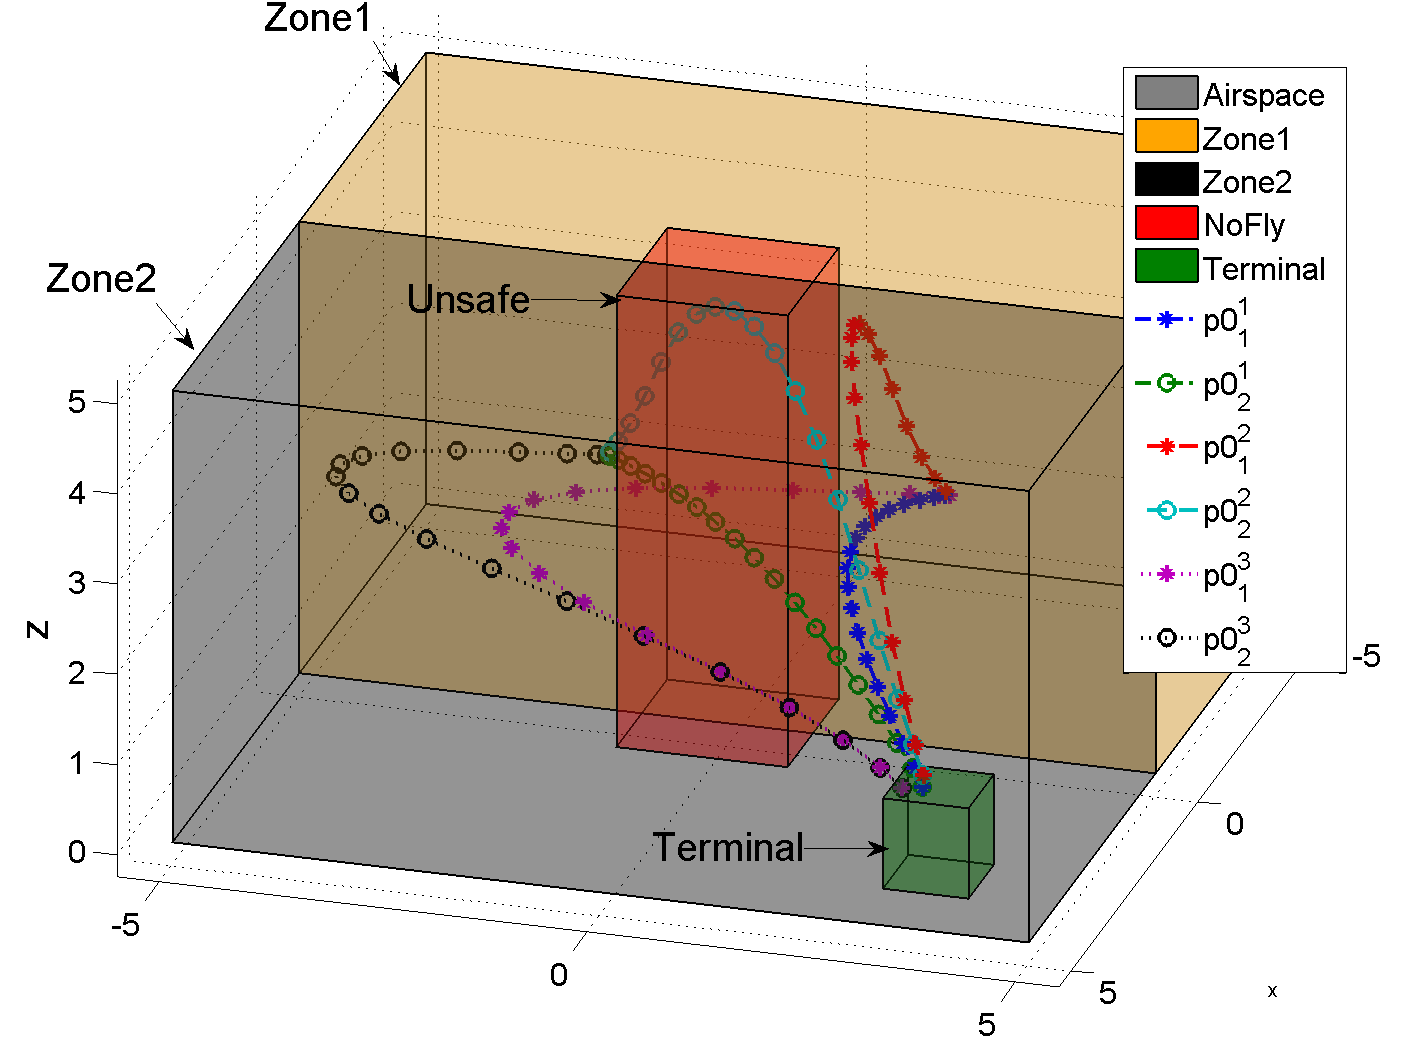
\includegraphics[width=0.49\textwidth]{figures/QuadInitTrajs_scissored}
%\vspace{-10pt}
%\caption{{\small The airspace with the corresponding sets, and initial trajectories for the two quad-rotors. Note, all 3 initial trajectories violate the specification, and the $\text{Airspace}$ is the union of $\text{Zone}_1$ and $\text{Zone}_2$. Here, $q0_{i}^j$ refers to the positions of the $i^{th}$ initial trajectory for the $j^{th}$ quadrotor.}}
%\label{fig:quad_init}
%\vspace{-10pt}
%\end{figure}
%Fig.\ref{fig:quad_init} shows the initial trajectories for both the quadrotors in the given air-space, neither of which satisfy the specification $\formula$. 

Fig.\ref{fig:quad_ssqp} shows the three trajectories obtained after applying SR-SQP,
with the three initial trajectories as initial guesses for the optimizations. 
%\todo[inline]{use the names of the methods, here, SR-SQP} 
%\todo[inline]{it's either a trajectory or a point. the reader can't peer into your head and see that you're thinking about them in the ssame way. Stick to one nomenclature, "initial trajectory". moreover, we've already explained above what an initial rajectory is, so we don't have to keep explaining that it initializes the optim.}
%for the optimization, respectively. 
All three trajectories obtained by SR-SQP satisfy the specification $\formula$. 
To avoid visual clutter, we do not show the trajectories obtained from the other two methods on the figure.
Instead, we summarize the results in Table \ref{tbl:opt_performance} which shows the true robustness of the three initial trajectories, and the true robustness for the trajectories obtained via the three methods, SR-SQP, SA, and R-SQP.In order to keep the study easy to interpret, we use two quad-rotors, but it is straight forward to scale the specification and the optimization to account for more. 

%Our method, SQP with Smooth Robustness (SR-SQP)
%\todo[inline]{define once, use forever: SR-SQP}, 
%results in trajectories with the highest robustness.
%SA, with an upper limit of 30,000 function evaluations, results in only one trajectory that satisfies $\formula$. 
%SQP on robustness 
%\todo[inline]{chicken on rice. R-SQP}
%results in trajectories that satisfy $\formula$ from all 3 initial trajectories. 
%R-SQP consistently returns lower values of robustness than SR-SQP, but also from three very different initial trajectories, 
%\todo[inline]{"very" initial?}
%\todo[inline]{re-organize: SR-SQP and R-SQP satisfies the spec every time, SA only once.
%	\\ SR-SQP gives highest robustness values, higher than R-SQP.
%	\\ observations below about getting stuck at local minima due to non-diff. }
%results in trajectories with the same robustness value $0.1798$. 

\textbf{Analysis.} It is seen that SR-SQP and R-SQP satisfy $\formula$ for all instances, while SA satisfies it only once.
Note that in all three cases, R-SQP results in trajectories with the same robustness value. 
We conjecture that this is because R-SQP is getting stuck at local minima at points of non-differentiability of the objective, as illustrated in Example \ref{ex:cluster nondiff}.
On further investigation, we also noticed that the robustness value achieved is due to the segment of the $\formula$ corresponding to $\eventually_{[0,N]}(q_2 \in \text{Terminal})$. R-SQP does not drive the trajectory (for quad-rotor 2) deeper inside the set $\text{Terminal}$, unlike the proposed approach, SR-SQP, even though the minimum separation property is far from being violated. This lends credence to our hypothesis of SQP terminating on a local minima, which is the flag MATLAB's optimization gives.

%\todo[inline]{this last discussion is important. break down your sentences, clarify it, take it easy. you've done the work, don't rush the explanation.}


\begin{figure}[t]
\centering
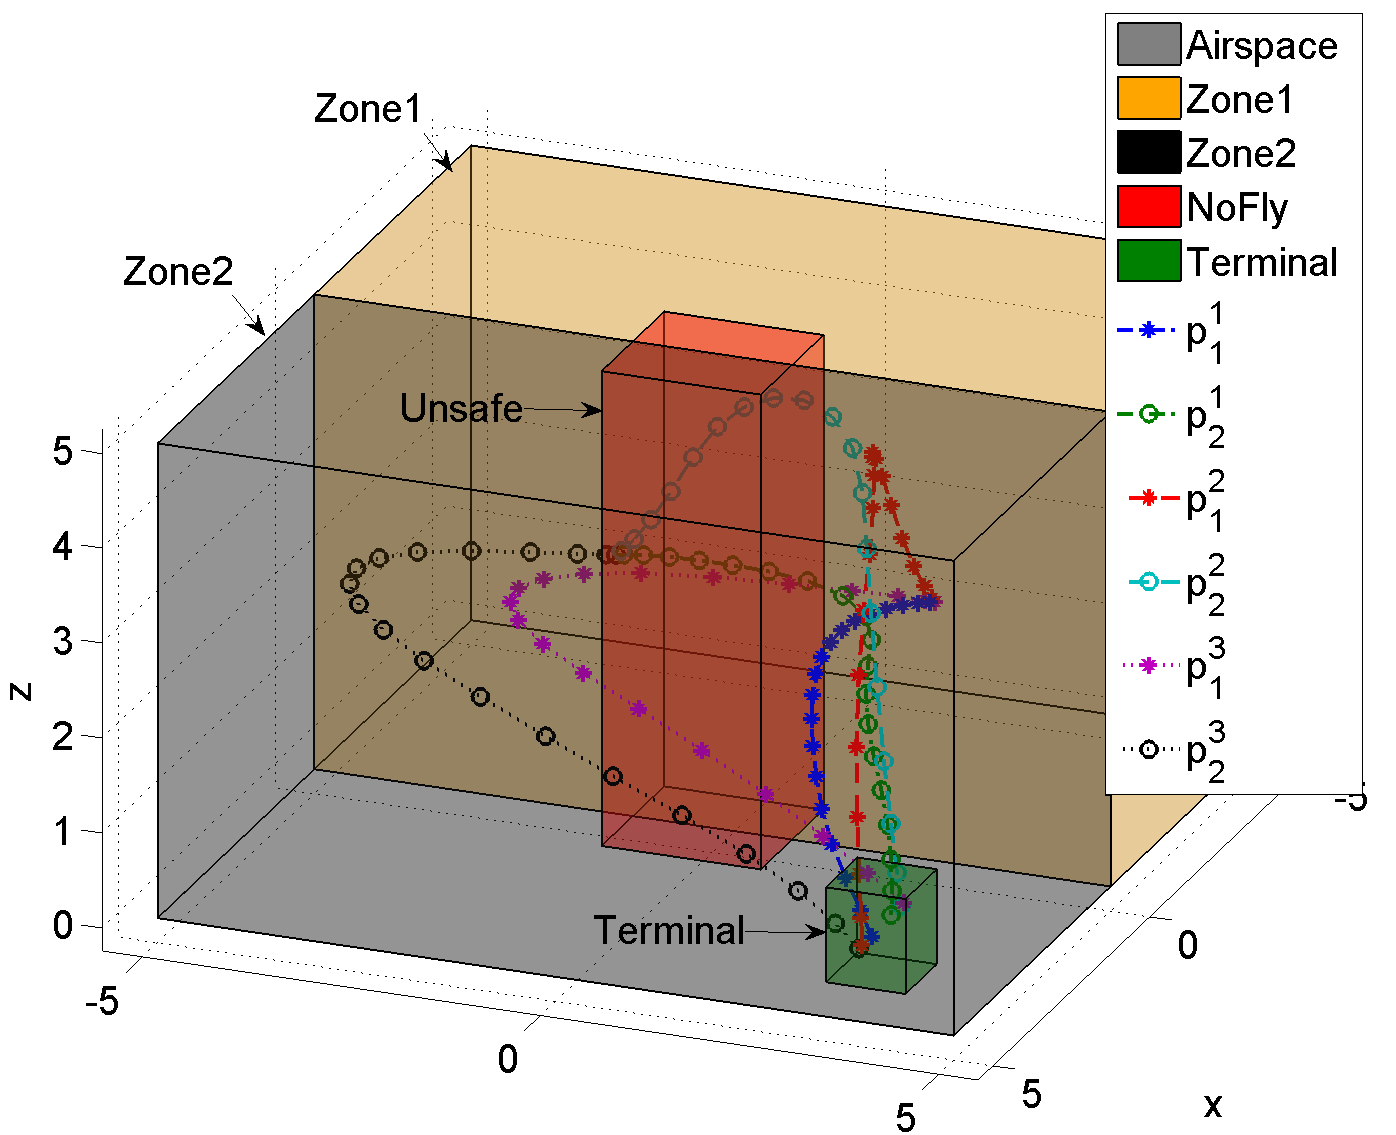
\includegraphics[width=0.49\textwidth]{figures/QuadTrajs_scissored}
\vspace{-10pt}
\caption{{\small Trajectories obtained via SQP on smooth robustness, with three different initial trajectories acting as initial solutions for the SQP. Note, all 3 trajectories satisfy $\formula$. Here, $q_{i}^j$ refers to the positions of the $i^{th}$ initial trajectory for the $j^{th}$ quadrotor. Consider $q_{1}^1$ and $q_{2}^1$, the first trajectory for the two quad-rotors. The second quad-rotor swerves around the obstacle and reaches $\text{Terminal}$, while the first quad-rotor swerves towards $\text{Unsafe}$, without violating $\formula$, in order to maintain a safe distance with the other quad-rotor while reaching $\text{Terminal}$. This results in the two quad-rotors satisfying $\formula$. Similar behavior is seen with the other two trajectories as well. A real-time playback of trajectories can be seen in \protect\url{http://bit.ly/2dY4xjw}.}}
\vspace{-10pt}
\label{fig:quad_ssqp}
\end{figure}


%
\begin{table}[htb]
\small
\begin{center}
\caption{{\small Robustness of final trajectory $\sstraj^*$ for three optimization runs with different initial trajectories.}}
\vspace{-10pt}
\label{tbl:opt_performance}
\begin{tabular} {|c|c|c|c|c|}
	\hline
	\textbf{Run} & $\rob(\sstraj_0) $ &SR-SQP $\rob(\sstraj^*) /\srob$ & SA: $\rob(\sstraj^*)$ & R-SQP: $\rob(\sstraj^*)$\\ \hline
	1 & -0.8803 & \textbf{0.2985} /\,0.2460 & -0.2424 & 0.1798 \\ \hline
	2 & -0.7832 & \textbf{0.3255} /\,0.3103 & -0.5861 & 0.1798 \\ \hline
	3 & -0.0399 & \textbf{0.2967} /\,0.2652 & 0.0854 & 0.1798 \\ \hline
\end{tabular}	
\end{center}
\vspace{-20pt}
\end{table}





\subsection{Discussion}
%\todo[inline]{skipping fr now}
With two case studies on dynamic systems, we show the applicability and consistently good performance of SOP (our method), which outperforms both SA R-SQP and BluSTL, which does not scale well enough to solve the second case study. For every instance we covered, SOP finds trajectories that satisfy the specification, while the other methods do not always do so.

%Also, while in the first case study, R-SQP, in the second case study, simulated annealing cannot find trajectories that satisfy the specification from two of the three initial trajectories (used as initial solutions for optimization). Our method on the other hand, successfully finds a trajectory that satisfies the specification, while resulting in the best robustness value achieved across all examples considered. 

While we solve the control problem in a single-shot, finite horizon manner, in general, for a real-time implementation, the problem can be solved in a receding horizon manner (similar to \cite{PantAMNDM15_Anytime}, \cite{Jain2016}). Or, it can be solved in a manner where the state and actions of the past are stored an added as constraints at each time step while the look-ahead horizon of the optimization shrinks (similar to \cite{Raman14_MPCSTL}). This will be explored further in future work. We have shown previously \cite{PantAMNDM15_Anytime} that control of an actual quad-rotor with the dynamics in \eqref{eq:quad_dyn} is possible on a low computation power platform. The control algorithm there involved solving multiple quadratic programs at even higher sampling rates ($20Hz$), in a receding horizon manner. Future work will include a C implementation of SOP, which will allow us to experiment on real platforms, like the aforementioned quad-rotors.
%Since all implementations were done in MATLAB, the focus was not real-time applicability of the proposed method. For the first case study, where the dynamics are slow, our method should still be applicable ($\sim 20s$) of execution time (compared to $\sim 5 \text{ mins}$ for SA). For the second case study a MATLAB implementation is infeasible due to the very fast dynamics and sampling times involved. We have shown previously in \cite{PantAMNDM15_Anytime} that control of a real quad-rotor with the dynamics in \eqref{eq:quad_dyn} is possible on a low computation power platform while solving multiple quadratic programs at even higher sampling rates ($20Hz$). With this in mind, we expect a C/C++ implementation of SQP (and the smooth robustness function) should allow us to implement our method on such a system. Ongoing work focuses on a general interpreter for formulae to generate corresponding smooth robustness functions, as well as their derivatives.
%\addtolength{\textheight}{-12cm}   % This command serves to balance the column lengths
% on the last page of the document manually. It shortens
% the textheight of the last page by a suitable amount.
% This command does not take effect until the next page
% so it should come on the page before the last. Make
% sure that you do not shorten the textheight too much.
\section*{ACKNOWLEDGMENT}

The authors would like to thank 
\bibliographystyle{plain}
\bibliography{iccps2017,hscc17,hscc2016,fainekos_bibrefs}
\end{document}